
%(BEGIN_QUESTION)
% Copyright 2011, Tony R. Kuphaldt, released under the Creative Commons Attribution License (v 1.0)
% This means you may do almost anything with this work of mine, so long as you give me proper credit

Suppose a digital temperature measurement system is not functioning as it should.  The ADC is outputting a count value of 002 (hex) when the sensor is known to be at a temperature of 20 degrees Celsius (room temperature).  The sensor is an RTD: a variable-resistance device which is supposed to be 100 ohms at 0 $^{o}$C and 138.5 ohms at 100 $^{o}$C, linearly proportional to temperature.  The analog input range of the ADC is 0 to 0.5 volts DC.  Your first diagnostic test is to check the voltage between test points {\bf G} and {\bf H}, and there you measure 5.08 volts DC:

$$\includegraphics[width=15.5cm]{i02173x01.eps}$$

Identify the likelihood of each specified fault for this circuit.  Consider each fault one at a time (i.e. no coincidental faults), determining whether or not each fault could independently account for {\it all} measurements and symptoms in this circuit.

% No blank lines allowed between lines of an \halign structure!
% I use comments (%) instead, so that TeX doesn't choke.

$$\vbox{\offinterlineskip
\halign{\strut
\vrule \quad\hfil # \ \hfil & 
\vrule \quad\hfil # \ \hfil & 
\vrule \quad\hfil # \ \hfil \vrule \cr
\noalign{\hrule}
%
% First row
{\bf Fault} & {\bf Possible} & {\bf Impossible} \cr
%
\noalign{\hrule}
%
% Another row
RTD failed open &  &  \cr
%
\noalign{\hrule}
%
% Another row
RTD failed shorted &  &  \cr
%
\noalign{\hrule}
%
% Another row
Wire broken open between points {\bf C} and {\bf E} &  &  \cr
%
\noalign{\hrule}
%
% Another row
Wire broken open between points {\bf C} and {\bf A} &  &  \cr
%
\noalign{\hrule}
%
% Another row
Wire broken open between points {\bf D} and {\bf B} &  &  \cr
%
\noalign{\hrule}
%
% Another row
Wire broken open between points {\bf D} and {\bf F} &  &  \cr
%
\noalign{\hrule}
%
% Another row
Current source dead &  &  \cr
%
\noalign{\hrule}
} % End of \halign 
}$$ % End of \vbox

Finally, identify the {\it next} diagnostic test or measurement you would make on this system.  Explain how the result(s) of this next test or measurement help further identify the location and/or nature of the fault.

\vskip 20pt \vbox{\hrule \hbox{\strut \vrule{} {\bf Suggestions for Socratic discussion} \vrule} \hrule}

\begin{itemize}
\item{} Calculate the ideal count value from the ADC at a sensor temperature of 100 $^{o}$C.
\item{} For those of you who have studied RTD temperature measurement, explain why we use {\it four} wires to connect the RTD to the measurement circuit, rather than just two wires.
\end{itemize}

\underbar{file i02173}
%(END_QUESTION)





%(BEGIN_ANSWER)

\noindent
{\bf Partial answer:}

% No blank lines allowed between lines of an \halign structure!
% I use comments (%) instead, so that TeX doesn't choke.

$$\vbox{\offinterlineskip
\halign{\strut
\vrule \quad\hfil # \ \hfil & 
\vrule \quad\hfil # \ \hfil & 
\vrule \quad\hfil # \ \hfil \vrule \cr
\noalign{\hrule}
%
% First row
{\bf Fault} & {\bf Possible} & {\bf Impossible} \cr
%
\noalign{\hrule}
%
% Another row
RTD failed open &  &  \cr
%
\noalign{\hrule}
%
% Another row
RTD failed shorted & $\surd$ &  \cr
%
\noalign{\hrule}
%
% Another row
Wire broken open between points {\bf C} and {\bf E} &  & $\surd$ \cr
%
\noalign{\hrule}
%
% Another row
Wire broken open between points {\bf C} and {\bf A} &  &  \cr
%
\noalign{\hrule}
%
% Another row
Wire broken open between points {\bf D} and {\bf B} &  &  \cr
%
\noalign{\hrule}
%
% Another row
Wire broken open between points {\bf D} and {\bf F} &  &  \cr
%
\noalign{\hrule}
%
% Another row
Current source dead & $\surd$ &  \cr
%
\noalign{\hrule}
} % End of \halign 
}$$ % End of \vbox


%(END_ANSWER)





%(BEGIN_NOTES)

% No blank lines allowed between lines of an \halign structure!
% I use comments (%) instead, so that TeX doesn't choke.

$$\vbox{\offinterlineskip
\halign{\strut
\vrule \quad\hfil # \ \hfil & 
\vrule \quad\hfil # \ \hfil & 
\vrule \quad\hfil # \ \hfil \vrule \cr
\noalign{\hrule}
%
% First row
{\bf Fault} & {\bf Possible} & {\bf Impossible} \cr
%
\noalign{\hrule}
%
% Another row
RTD failed open &  & $\surd$ \cr
%
\noalign{\hrule}
%
% Another row
RTD failed shorted & $\surd$ &  \cr
%
\noalign{\hrule}
%
% Another row
Wire broken open between points {\bf C} and {\bf E} &  & $\surd$ \cr
%
\noalign{\hrule}
%
% Another row
Wire broken open between points {\bf C} and {\bf A} & $\surd$ &  \cr
%
\noalign{\hrule}
%
% Another row
Wire broken open between points {\bf D} and {\bf B} & $\surd$ &  \cr
%
\noalign{\hrule}
%
% Another row
Wire broken open between points {\bf D} and {\bf F} &  & $\surd$ \cr
%
\noalign{\hrule}
%
% Another row
Current source dead & $\surd$ &  \cr
%
\noalign{\hrule}
} % End of \halign 
}$$ % End of \vbox


RTD resistance at 20 degrees Celsius = 107.7 ohms.  This should produce a voltage drop at the ADC of 269.25 mV, which in turn should produce a count value of 2205 or 89Dh.  

\vskip 10pt

The low count value suggests an abnormally low voltage at the ADC terminals E and F.  However, a broken wire between terminals C and E or between D and F is out of the question because the pull-up and pull-down resistors would cause the ADC to register full scale instead of low scale.  This leaves a shorted RTD, broken connection between current source and RTD, or a dead current source.

\vskip 10pt

A good ``next test'' would be to measure voltage at the RTD terminals (C and D) to determine whether or not it was receiving current from the source.

%Ideal count value at 100 $^{o}$C = 2836 = B14h

%INDEX Troubleshooting review: electric circuits

%(END_NOTES)


